\documentclass[a4paper]{amsart}
\usepackage{fullpage}
\setlength{\textwidth}{6.5in}
\usepackage[T1]{fontenc}
\usepackage{amsmath,amssymb,mathtools}
\usepackage{xcolor}
\usepackage{hyperref}
\usepackage{microtype,tikz}
\hypersetup{colorlinks=true,linkcolor=blue!45!black,citecolor=blue!45!black,
urlcolor=blue!45!black,pdftitle={Zeros of polyanalytic polynomials: linear bounds and explicit constructions},
pdfauthor={Antonio Lerario, Erik Lundberg, Teng Zhang}}
\newtheorem{thm}{Theorem}
\newtheorem{lem}[thm]{Lemma}
\newtheorem{prop}[thm]{Proposition}
\newtheorem{cor}[thm]{Corollary}
\newtheorem{problem}[thm]{Problem}
\newtheorem{conjecture}[thm]{Conjecture}
\theoremstyle{remark}
\newtheorem{rem}[thm]{Remark}
\newcommand{\C}{\mathbb C}
\newcommand{\R}{\mathbb R}
\newcommand{\Q}{\mathbb Q}
\newcommand{\CP}{\mathbb {CP}}
\newcommand{\eps}{\varepsilon}
\newcommand{\Nzero}{N}
\DeclareMathOperator{\Rea}{Re}
\DeclareMathOperator{\Ima}{Im}
\DeclareMathOperator{\rank}{rank}
\DeclareMathOperator{\sgn}{sgn}
\DeclareMathOperator{\sech}{sech}
\DeclareMathOperator{\csch}{csch}
\title[The Chebyshev example in conjugate degree one]{The Chebyshev construction in conjugate degree one}
\hypersetup{pdftitle={The Chebyshev construction in conjugate degree one}}
\author{Antonio Lerario}
\author{Erik Lundberg}
\author{Teng Zhang}
\date{October 5, 2026}
\begin{document}
\maketitle

The fact that \(T_1(z)=z\) is linear does not prevent the Chebyshev
construction from attaining \(3n-2\) zeros. The additional roots
come from the nonreal branches of \(\Ima T_n=0\). This note gives
a complete count and an explicit coefficient valid in every degree.
The count is the sharp bound proved by Khavinson and
\'{S}wi\k{a}tek \cite{KS03} and attained in Geyer's construction
\cite{Gey08}.

For a complex-valued map \(F\), let \(N(F)\) be its number of distinct
zeros. A zero is nondegenerate when the real differential is invertible.
The Chebyshev polynomial \(T_n\) is defined by
\(T_n(\cos\theta)=\cos(n\theta)\).

\begin{thm}\label{cor:explicit}
For every \(n\ge2\), the polynomial
\(p_n(z)=z-iT_n(z)/n^2\) satisfies
\(\#\{z:p_n(z)=\bar z\}=3n-2\), and every zero of
\(p_n(z)-\bar z\) is nondegenerate.
\end{thm}

\section{The real-level curves}
The identity \(T_n(\cos\zeta)=\cos(n\zeta)\) holds for complex
\(\zeta\), by the polynomial recurrence for \(T_n\).
Every point of the upper half-plane has a unique representation
\begin{equation}\label{eq:coordinates}
 z=\cos(\theta-it)=\cos\theta\cosh t+i\sin\theta\sinh t,
 \qquad 0<\theta<\pi,\quad t>0.
\end{equation}
Indeed, of the two solutions of \(\xi+\xi^{-1}=2z\), exactly one
has modulus greater than one. Its imaginary part is positive,
and writing it as \(e^{t+i\theta}\) gives \eqref{eq:coordinates}.
The differential is nonsingular: its determinant is
\(-(\sin^2\theta+\sinh^2t)<0\).
Since \(\Ima T_n(z)=\sin(n\theta)\sinh(nt)\), the nonreal upper
branches of the real-level set are
\begin{equation}\label{eq:branches}
 z_j(t)=\cos\theta_j\cosh t+i\sin\theta_j\sinh t,\qquad
 \theta_j=\frac{j\pi}{n},\quad 1\le j<n,\quad t>0.
\end{equation}
The remaining branches are their complex conjugates and the real
axis. On the \(j\)-th branch, \(T_n(z_j(t))=(-1)^j\cosh(nt)\).

\section{A complete count when the conjugate degree is one}
For every real \(a\), one has \(\Ima T_1(z-a)=\Ima z\).
We therefore study \(\eps T_n(z)-2\Ima z\). Put
\(\phi_n(t)=\sinh t/\cosh(nt)\) for \(t>0\).
Its logarithmic derivative is
\(\coth t-n\tanh(nt)\), whose derivative is
\(-\csch^2t-n^2\sech^2(nt)<0\).
The logarithmic derivative tends to \(+\infty\) at zero and to
\(1-n<0\) at infinity. Thus there is a unique \(t_n>0\) satisfying
\begin{equation}\label{eq:tn}
 \coth t_n=n\tanh(nt_n).
\end{equation}
The function \(\phi_n\) increases on \((0,t_n)\), decreases on
\((t_n,\infty)\), and tends to zero at both ends.
Define \(b_{n,j}=2\sin(j\pi/n)\phi_n(t_n)\), for \(1\le j<n\).

\begin{prop}\label{prop:allparameters}
For \(n\ge2\) and \(\eps>0\), let
\(f_{n,\eps}(z)=\eps T_n(z)-2\Ima z\). Then
\begin{equation}\label{eq:parametercount}
 N(f_{n,\eps})=
 n+2\#\{1\le j<n:\eps<b_{n,j}\}
   +\#\{1\le j<n:\eps=b_{n,j}\}.
\end{equation}
Every zero is nondegenerate unless \(\eps=b_{n,j}\) for some \(j\).
At such a parameter there is exactly one degenerate zero for
each index \(j\) with \(\eps=b_{n,j}\).
\end{prop}

\begin{proof}
On the real axis, \(f_{n,\eps}\) has the \(n\) simple zeros of \(T_n\).
At each such point \(x\), its Jacobian is \(\eps^2T_n'(x)^2>0\).
On the upper branch \(z_j(t)\) in \eqref{eq:branches},
its real part vanishes precisely when
\(\eps(-1)^j=2\sin\theta_j\phi_n(t)\).
On the reflected lower branch, the corresponding equation is
\(\eps(-1)^j=-2\sin\theta_j\phi_n(t)\).
Only the upper branch is possible for even \(j\), and only the lower
branch for odd \(j\). On the selected branch, the equation reduces to
\begin{equation}\label{eq:onecurve}
 \eps=2\sin\theta_j\,\phi_n(t).
\end{equation}
The monotonicity established before \eqref{eq:tn} gives two, one,
or no solutions according as \(\eps<b_{n,j}\),
\(\eps=b_{n,j}\), or \(\eps>b_{n,j}\). This proves
\eqref{eq:parametercount}.

The derivative of the imaginary part in the transverse
\(\theta\)-direction is, up to sign,
\(\eps n(-1)^j\sinh(nt)\ne0\). Along the selected branch, the
derivative of the real part at a zero is a nonzero factor times
\(\phi_n'(t)\). In the regular coordinates \eqref{eq:coordinates},
these derivatives prove nondegeneracy except at \(t=t_n\).
At \(t_n\), the differential has rank one. Moreover,
\(\phi_n''(t_n)<0\), because the logarithmic derivative is strictly
decreasing. The two roots of \eqref{eq:onecurve} therefore meet in a
quadratic tangency, and the stated degenerate zeros are the only ones.
\end{proof}

We now prove the explicit assertion of Theorem~\ref{cor:explicit}.
The minimum of the \(b_{n,j}\) is \(b_{n,1}\), and
\begin{equation}\label{eq:threshold}
 b_{n,1}\ge
 \frac{2\sin(\pi/n)\sinh(1/n)}{\cosh1}
 \ge \frac{4}{n^2\cosh1}>\frac1{n^2}.
\end{equation}
Here \(\sin(\pi/n)\ge2/n\), \(\sinh(1/n)\ge1/n\), and
\(\cosh1<4\). Equations~\eqref{eq:parametercount} and
\eqref{eq:threshold} show that \(f_{n,1/n^2}\) has \(n+2(n-1)\)
nondegenerate zeros. Finally,
\(-if_{n,1/n^2}=z-iT_n(z)/n^2-\bar z=p_n(z)-\bar z\).
Multiplication by \(-i\) preserves zeros and nondegeneracy, completing
the proof.

The location of the additional roots explains why the linearity
of \(T_1\) does not reduce the count. On every selected branch,
one solution of \eqref{eq:onecurve} approaches \(t=0\), and the
other approaches infinity as \(\eps\) decreases to zero.
Thus there are \(n-1\) roots near the real critical points of \(T_n\)
and \(n-1\) roots escaping to infinity, in addition to its \(n\)
real roots.

Figure~\ref{fig:chebyshev} illustrates the count when \(n=5\).

\begin{figure}[htbp]
\centering
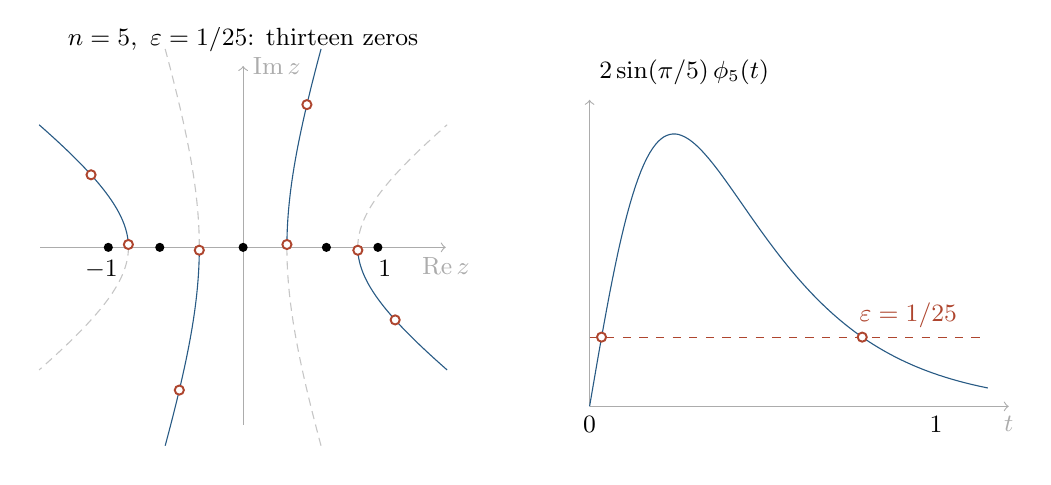
\begin{tikzpicture}[font=\small]
\definecolor{curveblue}{RGB}{40,90,132}
\definecolor{rootred}{RGB}{174,69,46}
\begin{scope}[x=1.8cm,y=1.8cm]
\clip (-1.52,-1.48) rectangle (1.64,1.55);
\draw[gray!65,->] (-1.43,0)--(1.43,0) node[below] {\(\Rea z\)};
\draw[gray!65,->] (0,-1.25)--(0,1.28) node[right] {\(\Ima z\)};
\node at (0,1.47) {\(n=5,\ \eps=1/25\): thirteen zeros};
\draw[curveblue,thin,domain=0:1.18,samples=90,variable=\t] plot ({cos(36.0)*(exp(\t)+exp(-\t))/2},{-1*sin(36.0)*(exp(\t)-exp(-\t))/2});
\draw[gray!45,densely dashed,thin,domain=0:1.18,samples=90,variable=\t] plot ({cos(36.0)*(exp(\t)+exp(-\t))/2},{1*sin(36.0)*(exp(\t)-exp(-\t))/2});
\draw[curveblue,thin,domain=0:1.18,samples=90,variable=\t] plot ({cos(72.0)*(exp(\t)+exp(-\t))/2},{1*sin(72.0)*(exp(\t)-exp(-\t))/2});
\draw[gray!45,densely dashed,thin,domain=0:1.18,samples=90,variable=\t] plot ({cos(72.0)*(exp(\t)+exp(-\t))/2},{-1*sin(72.0)*(exp(\t)-exp(-\t))/2});
\draw[curveblue,thin,domain=0:1.18,samples=90,variable=\t] plot ({cos(108.0)*(exp(\t)+exp(-\t))/2},{-1*sin(108.0)*(exp(\t)-exp(-\t))/2});
\draw[gray!45,densely dashed,thin,domain=0:1.18,samples=90,variable=\t] plot ({cos(108.0)*(exp(\t)+exp(-\t))/2},{1*sin(108.0)*(exp(\t)-exp(-\t))/2});
\draw[curveblue,thin,domain=0:1.18,samples=90,variable=\t] plot ({cos(144.0)*(exp(\t)+exp(-\t))/2},{1*sin(144.0)*(exp(\t)-exp(-\t))/2});
\draw[gray!45,densely dashed,thin,domain=0:1.18,samples=90,variable=\t] plot ({cos(144.0)*(exp(\t)+exp(-\t))/2},{-1*sin(144.0)*(exp(\t)-exp(-\t))/2});
\fill[black] (0.951056516,0.000000000) circle (1.65pt);
\fill[black] (0.587785252,0.000000000) circle (1.65pt);
\fill[black] (0.000000000,0.000000000) circle (1.65pt);
\fill[black] (-0.587785252,0.000000000) circle (1.65pt);
\fill[black] (-0.951056516,0.000000000) circle (1.65pt);
\fill[draw=rootred,fill=white,line width=.7pt] (0.809499276,-0.020298778) circle (1.65pt);
\fill[draw=rootred,fill=white,line width=.7pt] (1.072767415,-0.511849819) circle (1.65pt);
\fill[draw=rootred,fill=white,line width=.7pt] (0.309086081,0.020111885) circle (1.65pt);
\fill[draw=rootred,fill=white,line width=.7pt] (0.450074280,1.007091018) circle (1.65pt);
\fill[draw=rootred,fill=white,line width=.7pt] (-0.309086081,-0.020111885) circle (1.65pt);
\fill[draw=rootred,fill=white,line width=.7pt] (-0.450074280,-1.007091018) circle (1.65pt);
\fill[draw=rootred,fill=white,line width=.7pt] (-0.809499276,0.020298778) circle (1.65pt);
\fill[draw=rootred,fill=white,line width=.7pt] (-1.072767415,0.511849819) circle (1.65pt);
\node[below] at (-1,-.025) {\(-1\)};
\node[below] at (1,-.025) {\(1\)};
\end{scope}
\begin{scope}[shift={(4.4cm,-2.02cm)},x=4.4cm,y=22cm]
\draw[gray!65,->] (0,0)--(1.21,0) node[below] {\(t\)};
\draw[gray!65,->] (0,0)--(0,.177);
\node[anchor=south west] at (0,.18) {\(2\sin(\pi/5)\,\phi_5(t)\)};
\draw[curveblue,domain=0:1.15,samples=140,variable=\t] plot (\t,{2*sin(36)*(exp(\t)-exp(-\t))/(exp(5*\t)+exp(-5*\t))});
\draw[rootred,dashed] (0,.04)--(1.15,.04);
\node[rootred,above] at (.92,.04) {\(\eps=1/25\)};
\fill[draw=rootred,fill=white,line width=.7pt] (0.034527483,.04) circle (1.65pt);
\fill[draw=rootred,fill=white,line width=.7pt] (0.787012851,.04) circle (1.65pt);
\node[below] at (0,0) {\(0\)};
\node[below] at (1,0) {\(1\)};
\end{scope}
\end{tikzpicture}
\caption{The degree-five example. Filled dots are the five real zeros;
open circles are the eight nonreal zeros. Solid curves are the selected
branches of \(\Ima T_5=0\); their conjugates are dashed.
The right panel shows the two intersections that occur on each
selected branch, here for \(j=1\) and \(j=4\).}
\label{fig:chebyshev}
\end{figure}


\begin{thebibliography}{Gey08}
\bibitem[Gey08]{Gey08}
L.~Geyer, \emph{Sharp bounds for the valence of certain harmonic polynomials},
Proc. Amer. Math. Soc. \textbf{136} (2008), no.~2, 549--555.
\href{https://doi.org/10.1090/S0002-9939-07-08946-0}{doi:10.1090/S0002-9939-07-08946-0}.

\bibitem[KS03]{KS03}
D.~Khavinson and G.~\'{S}wi\k{a}tek,
\emph{On the number of zeros of certain harmonic polynomials},
Proc. Amer. Math. Soc. \textbf{131} (2003), no.~2, 409--414.
\href{https://doi.org/10.1090/S0002-9939-02-06476-6}{doi:10.1090/S0002-9939-02-06476-6}.

\end{thebibliography}
\end{document}
